\documentclass[margin=3mm]{standalone}
\usepackage{tikz}
\usetikzlibrary{shapes, arrows}

\tikzstyle{startstop} = [rectangle, rounded corners, minimum width=2cm, minimum height=1cm, text centered, draw=black, text=white, fill=black!80]
\tikzstyle{statement} = [rectangle, minimum width=4cm, minimum height=1cm, text centered, draw=black, fill=blue!20]
\tikzstyle{decision} = [rectangle, minimum height=1cm, text centered, draw=black, fill=yellow!30]
\tikzstyle{edge} = [thick, ->, >=stealth]

\begin{document}
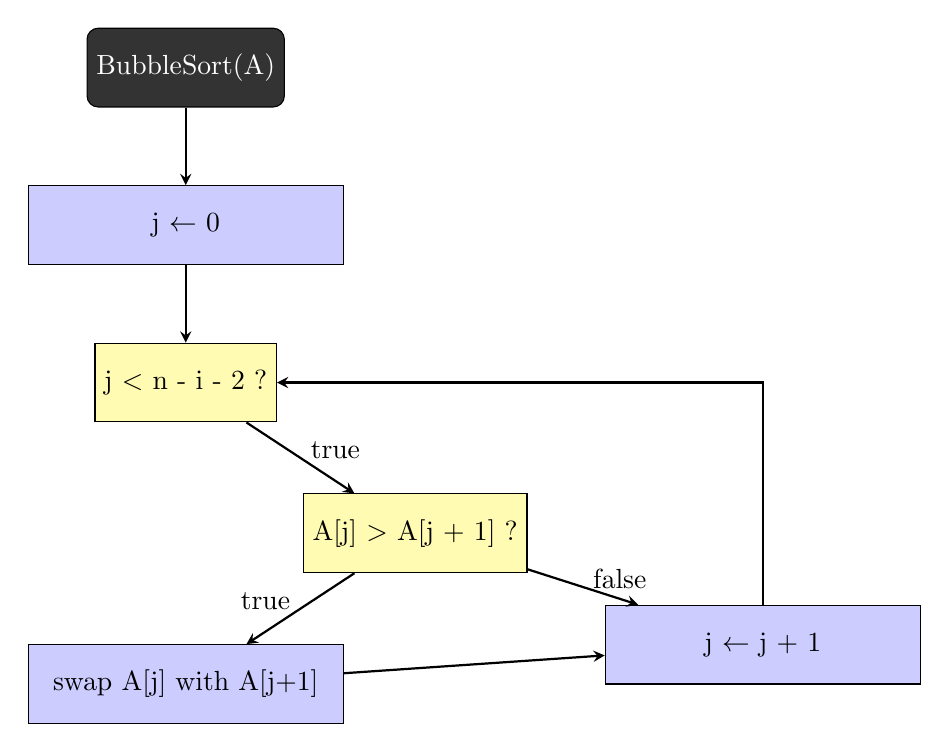
\begin{tikzpicture}[node distance=2cm]

\node (0) [startstop] {BubbleSort(A)};
\node (1) [statement, below of=0] {j $\gets$ 0};
\node (2) [decision, below of=1] {j $<$ n - i - 2 ?};
\node (3) [decision, yshift=-0.5cm, xshift=1.5cm, below right of=2] {A[j] $>$ A[j + 1] ?};
\node (4) [statement, yshift=-0.5cm, xshift=-1.5cm, below left of=3] {swap A[j] with A[j+1]};
\node (5) [statement, xshift=3cm, below right of=3] {j $\gets$ j + 1};

\draw [edge] (0) -- (1);
\draw [edge] (1) -- (2);
\draw [edge] (2) -- node[anchor=west, yshift=0.1cm]{true} (3);
\draw [edge] (3) -- node[anchor=west, yshift=0.1cm]{false} (5);
\draw [edge] (3) -- node[anchor=east, yshift=0.1cm]{true} (4);
\draw [edge] (4) -- (5);
\draw [edge] (5) |- (2);

\end{tikzpicture}
\end{document}